\section{Model Design}
This part of the research is the most important because the structure of the model and the model's parameters significantly impact the accuracy of hand gesture recognition. The choice of model depends on the dimensions and number of data as well as their nature. However, choosing model parameters requires trial and error, making the design process complicated and time-consuming [29]. The number of model parameters can also be one of the design variables, but this study's primary purpose is to maximize the model's accuracy in pattern recognition. 

Input data are labeled, so the present model is a supervised model. In traditional machine learning and classification methods, the model requires a section that extracts a series of features from the input signals. The classifier then divides the signals into different classes based on these features. The accuracy of these models strongly depends on the selected features. The deep CNN network, selected as the present classifier model, extracts high-level data features by convolutional layers. This feature extraction method, called feature learning, performs better than traditional hand-crafted features[30].

The model consists of a series of convolutional layers, a dense layer, and a SoftMax layer with eight neurons [31]. Each convolutional layer contains kernels of specified dimensions. These kernels move on the signal with a fixed step and extract the properties. In this research, rectified linear units (Relu) have been used as an activation function to prevent the Gradient vanishing phenomenon and improve the training speed [32]. The dimension of the kernels are 20 × 8, and their step size is one. The number of convolutional layers, the number of neurons of dense layer neurons, and  The number of kernels in each layer are the parameters whose optimal value will be calculated using the genetic algorithm. The last layer of this model consists of 8 neurons with the SoftMax activation function. 

A high value of the learning rate causes training to fluctuate and may not to be converged , and a low value reduces the convergence rate of the model. The learning rate choice also affects the number of epochs; the lower the learning rate, the higher the epochs. On the other hand, a high number of epochs may overfit the model [33]. Figure 2 shows that with a higher learning rate, the model converges faster, but at higher epochs, overfitting occurs. On the other hand, model training with a small learning rate requires higher processing power. According to the experimental results, the number of epochs is 30, the learning rate is 0.0001, and the Batch size is 65. Also, the activation functions and the kernel size in all layers are relu and 20 × 8.  These parameters can also be added to independent variables optimized by the genetic algorithm, but with each parameter's addition, the computation time will increase. Therefore, in this study, only the model structure parameters, including the number of convolutional layers, the number of kernels in each layer, and the number of dense layer's neurons, are considered independent variables. In this model, the Adaptive moment estimation optimizer is used to train the coefficients, the categorical cross-entropy is used as the error function, and The coefficients are initialized by the random uniform method [34,35].


\begin{figure}
    \centering
    \begin{subfigure}[b]{0.2\textwidth}
        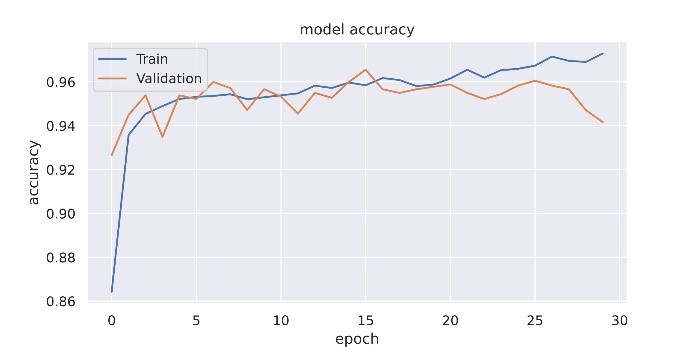
\includegraphics[width=\textwidth]{figures/lr/1.jpg}
    \end{subfigure}
    \begin{subfigure}[b]{0.2\textwidth}
        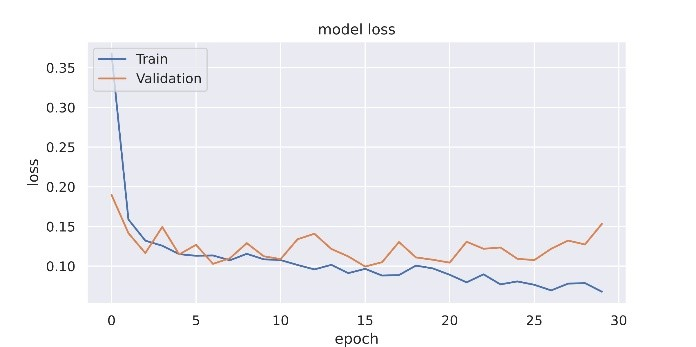
\includegraphics[width=\textwidth]{figures/lr/2.jpg}
    \end{subfigure}



    \begin{subfigure}[b]{0.2\textwidth}
        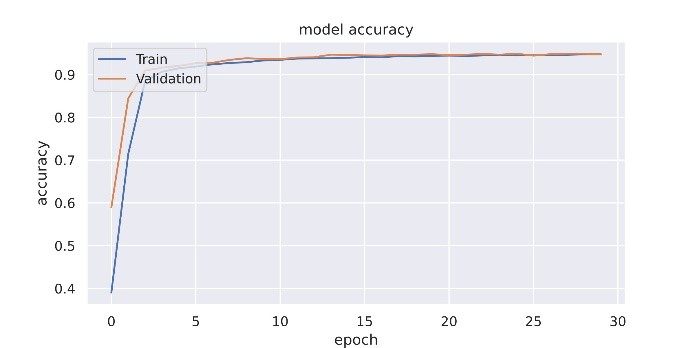
\includegraphics[width=\textwidth]{figures/lr/3.jpg}
    \end{subfigure}
    \begin{subfigure}[b]{0.2\textwidth}
        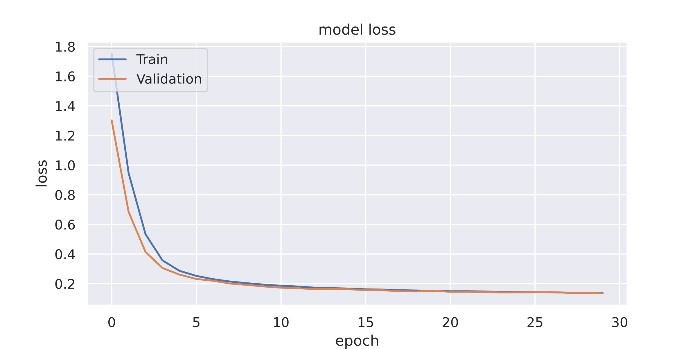
\includegraphics[width=\textwidth]{figures/lr/4.jpg}
    \end{subfigure}
    \caption{\centering
    Comparison of model accuracy and loss  for learning rate 0.0001 (top) and 0.00001 (bottom}
    \label{fig:lr_s}
\end{figure}